 \thispagestyle{gocconone}
\pagestyle{gocco}
\everymath{\color{gocco}}
\graphicspath{{../gocco/pic/}}
\blfootnote{$^1${\color[named]{gocco}Đại kiện tướng quốc tế.}}
\begingroup
\AddToShipoutPicture*{\put(0,616){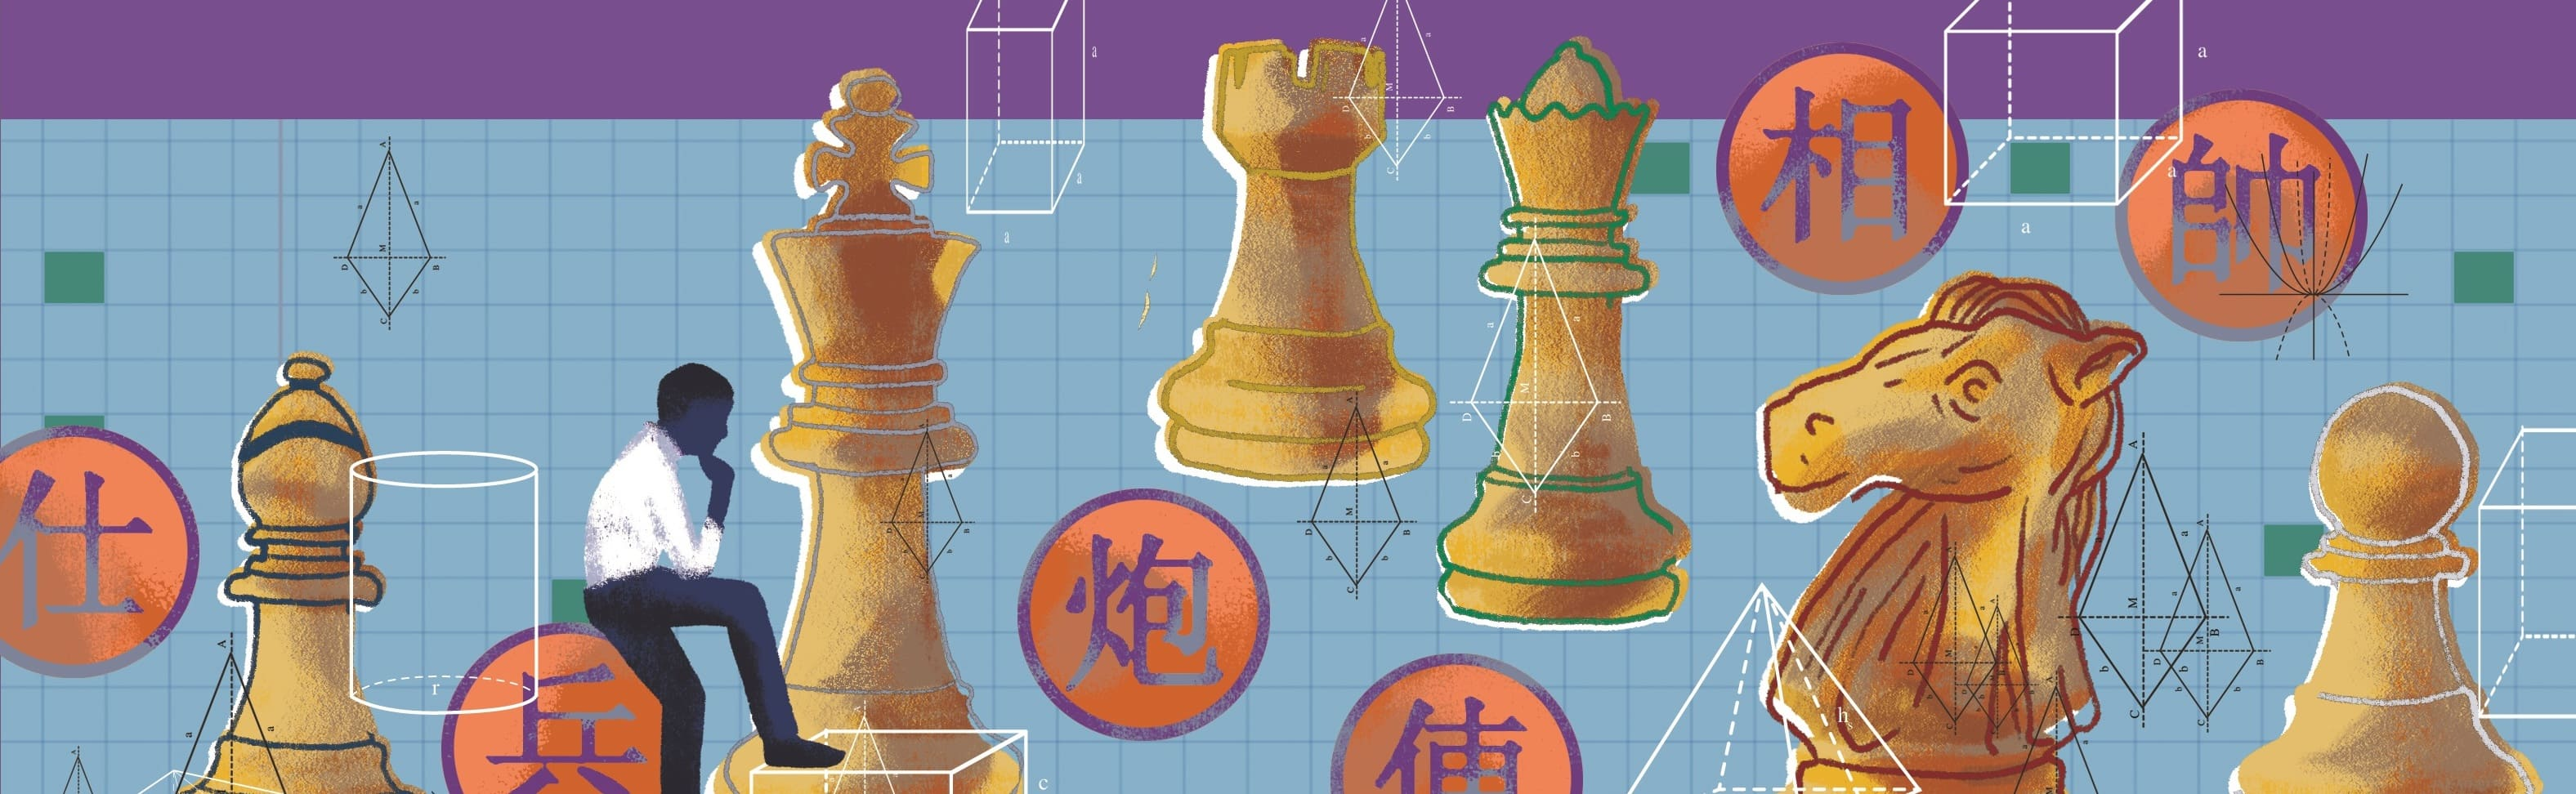
\includegraphics[width=19.3cm]{../bannergocco}}}
\AddToShipoutPicture*{\put(138,555){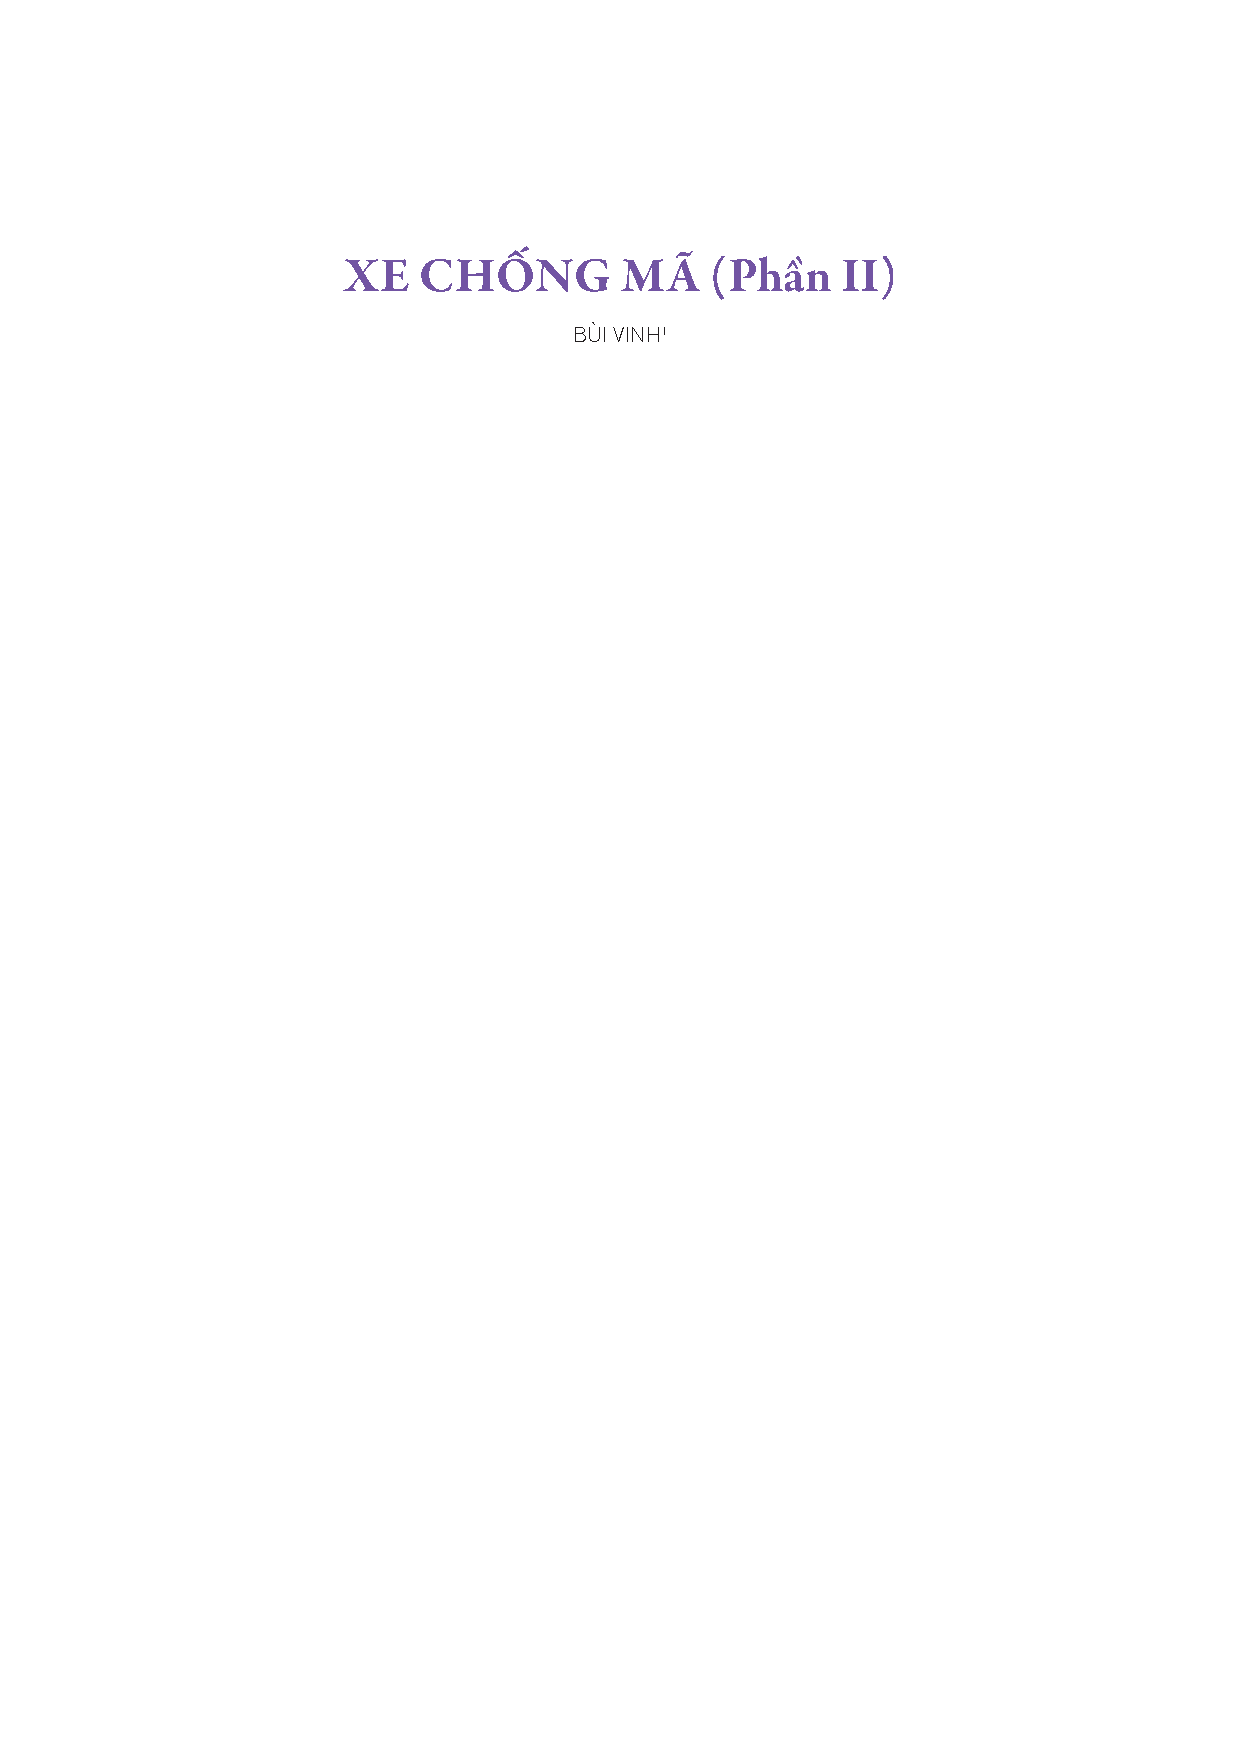
\includegraphics[scale=1]{../tieude5.pdf}}} 
\centering
\endgroup

\vspace*{155pt}
\begin{multicols}{2}
	Lý thuyết cơ bản của cờ tàn Xe chống Mã khi hai bên không còn Tốt thường được đánh giá là hòa cờ cơ bản. Nếu như Vua và Mã luôn đứng cạnh nhau hoặc ở giữa bàn cờ, bên có Xe không thể giành chiến thắng. Tuy nhiên trên thực tế rất nhiều các kỳ thủ rất mạnh cũng đôi khi mắc phải những sai lầm nghiêm trọng trong thi đấu dẫn đến thua cờ.
	\vskip 0.1cm
	Trong phần I bài viết này, chúng ta đã xem xét một số trường hợp khi Vua và Mã đối phương nằm ở hàng ngang cuối $1$ và $8$ hoặc ở cột $a$ và $h$. Trong các trường hợp Mã đứng sai vị trí hoặc đứng tách rời khỏi Vua của mình, cơ hội giành chiến thắng của bên có Xe sẽ dễ dàng rất nhiều.
	\vskip 0.1cm
	Chúng ta nghiên cứu một số ví dụ dưới đây. 
	\begin{center}
		\newgame
		\fenboard{6k1/8/5K2/R7/2n5/8/8/8 b Q - 0 1}
		\scalebox{0.85}\showboard
		\vskip 0.1cm
		\textit{\small\color{gocco}Hình $1$.}
	\end{center}
	\textbf{\color{gocco}$\pmb{1}$.Xa$\pmb{8+}$ Vh$\pmb{7}$ $\pmb{2}$.Xa$\pmb{7+}$ Vg$\pmb{8}$} [$2$...Vh$6$ $3$.Xa$4$ Me$3$ $4$.Xh$4\#$; $2$...Vh$8$ $3$.Xc$7$ Me$3$ $4$.Vg$6$]
	\vskip 0.1cm
	\textbf{\color{gocco}$\pmb{3}$.Xd$\pmb{7}$! (H$\pmb{5}$)} Kỹ thuật cơ bản của trắng lúc này là vừa đe dọa chiếu hết và tách Mã đen khỏi Vua. \textbf{\color{gocco}Me}$\pmb{3}$ [$3$...Vh$8$ $4$.Xd$4$ Mb$6$ $5$.Vf$7$; $3$...Mb$6$ $4$.Xd$4$ Vh$7$ $5$.Vf$7$ Vh$6$ $6$.Xd$6+$]
	\begin{center}
		\newgame
		\fenboard{6k1/3R4/5K2/8/2n5/8/8/8 b Q - 0 1}
		\scalebox{0.85}\showboard
		\vskip 0.1cm
		\textit{\small\color{gocco}Hình $2$.}
	\end{center}
	\begin{center}
		\newgame
		\fenboard{5k2/8/6K1/8/4R3/8/2n5/8 b Q - 0 1}
		\scalebox{0.85}\showboard
		\vskip 0.1cm
		\textit{\small\color{gocco}Hình $3$.}
	\end{center}
	\textbf{\color{gocco}$\pmb{4}$.Vg$\pmb{6}$ Vf$\pmb{8}$ $\pmb{5}$.Xd$\pmb{4}$ Mc$\pmb{2}$ $\pmb{6}$.Xe$\pmb{4}$} Xe trắng khống chế hoàn toàn các ô cờ di chuyển của Mã đen.  \textbf{\color{gocco}Ma}$\pmb{3}$ [$6$...Ma$1$ $7$.Vf$6$ Vg$8$ $8$.Xg$4+$ Vh$7$ $9$.Xg$7+$ Vh$8$ $10$.Vg$6$ Mc$2$ $11$.Xc$7$]
	\vskip 0.1cm
	\textbf{\color{gocco}$\pmb{7}$.Vf$\pmb{6}$!! Vg$\pmb{8}$ $\pmb{8}$.Xg$\pmb{4+}$ Vh$\pmb{7}$ $\pmb{9}$.Xg$\pmb{7+}$ Vh$\pmb{8}$} [$\pmb{9}$...Vh$\pmb{6}$ $\pmb{10}$.Xg$\pmb{3}$]
	\vskip 0.1cm
	\textbf{\color{gocco}$\pmb{10}$.Vg$\pmb{6}$ Mc$\pmb{4}$ $\pmb{11}$.Xe$\pmb{7}$} Trắng thắng
	\vskip 0.1cm
	Ví dụ tiếp theo cho thấy ngay cả khi Mã và bên yếu đứng cạnh nhau, nhưng vị trí Mã yếu vẫn có thể dẫn đến thua cờ. 
	\begin{center}
		\newgame
		\fenboard{7R/k7/2K5/n7/8/8/8/8 b Q - 0 1}
		\scalebox{0.85}\showboard
		\vskip 0.2cm
		\textit{\small\color{gocco}Hình $4$.}
	\end{center}
	\textbf{\color{gocco}$\pmb{1}$.Vb$\pmb{5}$ Mb$\pmb{7}$} [$1$...Mb$3$ $2$.Xd$8$ Vb$7$ $3$.Xd$1$]
	\vskip 0.1cm
	\textbf{\color{gocco}$\pmb{2}$.Xf$\pmb{8}$! Md$\pmb{6+}$ $\pmb{3}$.Vc$\pmb{6}$ Mc$\pmb{4}$} [ Phương án $3$...Mb$7$ $4$.Xf$7$ Va$8$ $5$.Vb$6$; $3$...Me$4$ $4$.Xf$7+$ Vb$8$ $5$.Xb$7+$ Va$8$ $6$.Xb$4$ Mf$6$ $7$.Xf$4$ Mh$5$ $8$.Xf$5$ Mg$3$ (\textit{$8$...Mg$7$ $9$.Xf$8+$ Va$7$ $10$.Xf$7+$}) $9$.Xf$3$ Me$4$ $10$.Vb$6$]
	\begin{center}
		\newgame
		\fenboard{k7/8/1K6/8/4n3/5R2/8/8 b Q - 0 1}
		\scalebox{0.85}\showboard
		\vskip 0.2cm
		\textit{\small\color{gocco}Hình $5$. Đen không thể ngăn cản nước chiếu hết ở hàng ngang số $8$.}
	\end{center}
	\textbf{\color{gocco}$\pmb{4}$.Xf$\pmb{4}$ Ma$\pmb{5+}$} [Phương án khác $4$...Md$2$ $5$.Xa$4+$ Vb$8$ $6$.Vb$6$ Xc$8$ $7$.Xf$4$ Mb$3$ $8$.Xf$3$ Md$2$ (\textit{$8$...Md$4$ $9$.Xc$3+$ Vb$8$ $10$.Xd$3$ Me$6$ $11$.Xd$6$}) $9$.Xc$3+$ Vb$8$ $10$.Xc$6$ Mb$3$ $11$.Xc$4$]
	\begin{center}
		\newgame
		\fenboard{1k6/8/1K6/8/2R5/1n6/8/8 b Q - 0 1}
		\scalebox{0.85}\showboard
		\vskip 0.2cm
		\textit{\small\color{gocco}Hình $6$. Mã đen bị hết nước đi.}
	\end{center}
	\textbf{\color{gocco}$\pmb{5}$.Vb$\pmb{5}$ Mb$\pmb{7}$ $\pmb{6}$.Xd$\pmb{4}$ Vb$\pmb{8}$ $\pmb{7}$.Va$\pmb{6}$!} Bằng các nước đi Vua khéo léo, Vua và Xe trắng phối hợp kiểm soát chặt chẽ các ô cờ di chuyển của Mã đen. Đồng thời không cho phép Mã đen có thời gian chuyển đến các có thể gỡ hòa như c$8$. Vc$7$ [Nếu $7$...Mc$5+$ $8$.Vb$6$ Me$6$ (\textit{$8$...Mb$7$ $9$.Xd$7$ Va$8$ $10$.Xh$7$}) $9$.Xd$6$]
	\begin{center}
		\newgame
		\fenboard{1k6/1n6/K7/8/3R4/8/8/8 b Q - 0 1}
		\scalebox{0.85}\showboard
		\vskip 0.2cm
		\textit{\small\color{gocco}Hình $7$.}
	\end{center}
	\begin{center}
		\newgame
		\fenboard{k7/1n5R/1K6/8/8/8/8/8 b Q - 0 1}
		\scalebox{0.85}\showboard
		\vskip 0.2cm
		\textit{\small\color{gocco}Hình $8$.}
	\end{center}
	\textbf{\color{gocco}$\pmb{8}$.Xc$\pmb{4+}$ Vb$\pmb{8}$ $\pmb{9}$.Xb$\pmb{4}$ Va$\pmb{8}$ $\pmb{10}$.Vb$\pmb{6}$! Vb$\pmb{8}$} [$10$...Md$6$ $11$.Xh$4$ Vb$8$ $12$.Xh$8+$ Mc$8+$ $13$.Mc$6$]
	\vskip 0.1cm
	\textbf{\color{gocco}$\pmb{11}$.Vc$\pmb{6}$ Va$\pmb{8}$ $\pmb{12}$.Xh$\pmb{4}$ Vb$\pmb{8}$} [$12$...Md$8+$ $13$.Vc$7$ Me$6+$ $14$.Vb$6$]
	\vskip 0.1cm
	\textbf{\color{gocco}$\pmb{13}$.Xh$\pmb{8+}$ Va$\pmb{7}$ $\pmb{14}$.Xh$\pmb{7}$ Va$\pmb{8}$ $\pmb{15}$.Vb$\pmb{6}$}
	\vskip 0.1cm
	\textit{Như vậy qua xem xét một số ví dụ, chúng ta thấy lý thuyết về Vua và Xe  chống Vua và Mã khi hai bên không còn Tốt hầu hết đều cho rằng đó là thế cờ hòa cơ bản. Tuy nhiên trên thực tế, nếu khi chơi các kỳ thủ không nắm chắc kiến thức vẫn có thể thua cờ.}
	\vskip 0.05cm
	\textbf{\color{gocco}Bài tập $\pmb{1}$:}
	\begin{center}
		\newgame
		\fenboard{8/8/8/1k1K4/8/6R1/5n2/8 b Q - 0 1}
		\scalebox{0.85}\showboard
		\vskip 0.2cm
		\textit{\small\color{gocco}Hình $9$. Trắng đi trước thắng.}
	\end{center}
	\textbf{\color{gocco}Bài tập $\pmb{2}$: (Reti, $\pmb{1929}$)}
	\begin{center}
		\newgame
		\fenboard{8/8/1k6/8/2KR4/8/5n2/8 b Q - 0 1}
		\scalebox{0.85}\showboard
		\vskip 0.2cm
		\textit{\small\color{gocco}Hình $10$. Trắng đi trước thắng.}
	\end{center}
	\textbf{\color{gocco}Bài tập $\pmb{3}$: (A. Karpov -- L. Ftacnik, Thessalonniki olympiad (men) $\pmb{1988}$)}
	\begin{center}
		\newgame
		\fenboard{3R4/8/8/6k1/2n1K3/8/8/8 b Q - 0 1}
		\scalebox{0.85}\showboard
		\vskip 0.2cm
		\textit{\small\color{gocco}Hình $11$. Trắng đi trước thắng.}
	\end{center}
%	\textbf{\color{gocco}Lời giải:}
%	\vskip 0.1cm
%	\textbf{\color{gocco}Bài $\pmb{1}$.
%	$\pmb{1}$.Vd$\pmb{4}$ Vb$\pmb{4}$ $\pmb{2}$.Xg$\pmb{2}$ Mh$\pmb{3}$} [$2$...Md$1$ $3$.Xd$2$]
%	\vskip 0.1cm
%	\textbf{\color{gocco}$\pmb{3}$.Ke$\pmb{3}$} Mã đen bị bắt.
%	\vskip 0.1cm
%	\textbf{\color{gocco}Bài $\pmb{2}$. 
%	$\pmb{1}$.Vc$\pmb{4}$ Vc$\pmb{6}$} [$1$...Mh$3$ $2$.Xg$4$ Mf$2$ $3$.Xh$4$]
%	\vskip 0.1cm
%	\textbf{\color{gocco}$\pmb{2}$.Xh$\pmb{4}$ Vd$\pmb{6}$ $\pmb{3}$.Vd$\pmb{4}$ Ve$\pmb{6}$ $\pmb{4}$.Ve$\pmb{3}$ Md$\pmb{1+}$ $\pmb{5}$.Vd$\pmb{2}$ Mb$\pmb{2}$} [$5$...Mf$2$ $6$.Ve$2$]
%	\vskip 0.1cm
%	\textbf{\color{gocco}$\pmb{6}$.Xb$\pmb{4}$}
%	\vskip 0.1cm
%	\textbf{\color{gocco}Bài $\pmb{3}$.
%	$\pmb{1}$.Xd$\pmb{4}$!! Mb$\pmb{6}$} [$1$...Mb$2$ $2$.Ve$3$ Vf$5$ $3$.Vd$2$ Ve$5$ $4$.Xb$4$]
%	\vskip 0.1cm
%	\textbf{\color{gocco}$\pmb{2}$.Ve$\pmb{5}$ Mc$\pmb{8}$ $\pmb{3}$.Ve$\pmb{6}$ Ma$\pmb{7}$ $\pmb{4}$.Vd$\pmb{7}$ Mb$\pmb{5}$} [$4$...Vf$5$ $5$.Xa$4$ Mb$5$ $6$.Xa$5$; $4$...Vg$6$ $5$.Xd$5$]
%	\vskip 0.1cm
%	\textbf{\color{gocco}$\pmb{5}$.Xd$\pmb{5+}$}
%	\vskip 0.1cm
%	$\pmb{1-0}$
%	
%	\vfill\null
\end{multicols}
\vspace*{-10pt}
\rule{1\linewidth}{0.1pt}
\begin{center}
	\textbf{\Large\color{gocco}LỜI GIẢI, ĐÁP ÁN}
\end{center}
\begin{multicols}{2}
	\textbf{\color{gocco}Góc cờ}
	\vskip 0.1cm
	\textbf{\color{gocco}Bài $\pmb{1}$.
				$\pmb{1}$.Vd$\pmb{4}$ Vb$\pmb{4}$ $\pmb{2}$.Xg$\pmb{2}$ Mh$\pmb{3}$} [$2$...Md$1$ $3$.Xd$2$]
	\vskip 0.1cm
	\textbf{\color{gocco}$\pmb{3}$.Ke$\pmb{3}$} Mã đen bị bắt.
	\vskip 0.1cm
	\textbf{\color{gocco}Bài $\pmb{2}$. 
				$\pmb{1}$.Vc$\pmb{4}$ Vc$\pmb{6}$} [$1$...Mh$3$ $2$.Xg$4$ Mf$2$ $3$.Xh$4$]
	\vskip 0.1cm
	\textbf{\color{gocco}$\pmb{2}$.Xh$\pmb{4}$ Vd$\pmb{6}$ $\pmb{3}$.Vd$\pmb{4}$ Ve$\pmb{6}$ $\pmb{4}$.Ve$\pmb{3}$ Md$\pmb{1+}$ $\pmb{5}$.Vd$\pmb{2}$ Mb$\pmb{2}$} [$5$...Mf$2$ $6$.Ve$2$]
	\vskip 0.1cm
	\textbf{\color{gocco}$\pmb{6}$.Xb$\pmb{4}$}
	\vskip 0.1cm
	\textbf{\color{gocco}Bài $\pmb{3}$.
				$\pmb{1}$.Xd$\pmb{4}$!! Mb$\pmb{6}$} [$1$...Mb$2$ $2$.Ve$3$ Vf$5$ $3$.Vd$2$ Ve$5$ $4$.Xb$4$]
	\vskip 0.1cm
	\textbf{\color{gocco}$\pmb{2}$.Ve$\pmb{5}$ Mc$\pmb{8}$ $\pmb{3}$.Ve$\pmb{6}$ Ma$\pmb{7}$ $\pmb{4}$.Vd$\pmb{7}$ Mb$\pmb{5}$} [$4$...Vf$5$ $5$.Xa$4$ Mb$5$ $6$.Xa$5$; $4$...Vg$6$ $5$.Xd$5$]
	\vskip 0.1cm
	\textbf{\color{gocco}$\pmb{5}$.Xd$\pmb{5+}$}
	\vskip 0.1cm
	$\pmb{1-0}$
\end{multicols}



